\documentclass[10pt,twocolumn,letterpaper]{article}

\usepackage{iccv}
\usepackage{times}
\usepackage{epsfig}
\usepackage{graphicx}
\usepackage{amsmath}
\usepackage{amssymb}
\usepackage{graphicx}

% ------ New Package Here ------
\usepackage{dblfloatfix}
\usepackage{subcaption}
\usepackage{bm}
\usepackage[pagebackref=true,breaklinks=true,letterpaper=true,colorlinks=true,bookmarks=true]{hyperref}
% ------------------------------

\makeatletter
\newcommand\footnoteref[1]{\protected@xdef\@thefnmark{\ref{#1}}\@footnotemark}
\makeatother


%---------MATH SYMBOLS NEW COMMANDS:--------------------------------------
\newcommand{\vectornorm}{|}

\newcommand{\diver}{\mathrm{div}}
\newcommand{\grad}{\mathrm{grad}}
\newcommand{\trace}{\mathrm{trace}}
\newcommand{\ud}{\mathrm{d}}

\newcommand{\mvec}[1]{\boldsymbol{#1}}
\newcommand{\matr}[1]{\mathrm{#1}}

\newcommand{\eye}{\mathrm{I}}
\newcommand{\img}{u}

\newcommand{\prob}[1]{\mathrm{p}\left( #1 \right)}

\newcommand{\bhat}{\widehat{\mvec{b}}}
\newcommand{\lamhat}{\widehat{\mvec{\lambda}}}
\newcommand{\eps}{\mvec{\varepsilon}}

%\newcommand{\norm}[1]{\left\Vert#1\right\Vert}
% \newcommand{\norm}[1]{\left \|#1 \right \|}
\newcommand{\norm}[1]{\left |#1 \right |}
\newcommand{\transp}{^\mathrm{T}}

\newcommand{\bu}{\boldsymbol{u}}
\newcommand{\bx}{\boldsymbol{x}}
\newcommand{\bp}{\boldsymbol{p}}

\newcommand{\be}{\boldsymbol{\varepsilon}}

\newcommand{\bv}{\boldsymbol{v}}
\newcommand{\mfsf}[0]{{\sc mfsf}}
\newcommand{\mfsfc}[0]{{\sc mfsf\em c}}
\newcommand{\mfsfdct}[0]{{\sc mfsf$_{\tt DCT}$}}
\newcommand{\mfsfpca}[0]{{\sc mfsf$_{\tt PCA}$}}
\newcommand{\mfsfid}[0]{{\sc mfsf$_{\tt I_{2F}}$}}
\newcommand{\mfsfcdct}[0]{{\sc mfsf\em c$_{\tt DCT}$}}
\newcommand{\mfsfcpca}[0]{{\sc mfsf\em c$_{\tt PCA}$}}
\newcommand{\mfsfcid}[0]{{\sc mfsf\em c$_{\tt I_{2F}}$}}


\newcommand{\cU}{\mathcal{U}}
\newcommand{\bU}{\boldsymbol{\mathcal{U}}}
\newcommand{\bE}{\boldsymbol{\mathcal{E}}}
\newcommand{\bI}{\boldsymbol{I}}
\newcommand{\bA}{\boldsymbol{A}}
\newcommand{\bb}{\boldsymbol{b}}
\DeclareMathOperator*{\argmin}{arg\,min}
\DeclareMathOperator*{\argmax}{arg\,max}


\newcommand{\bL}{\boldsymbol{L}}
\newcommand{\bM}{\boldsymbol{M}}

\newcommand{\R}{\mathbb{R}}

\newcommand{\Lone}{\mathbf{L}^1}
\newcommand{\Ltwo}{\mathbf{L}^2}


%----------------------------------------------------------------------------------------------------

% \iccvfinalcopy % *** Uncomment this line for the final submission

\def\iccvPaperID{1612} % *** Enter the ICCV Paper ID here
\def\httilde{\mbox{\tt\raisebox{-.5ex}{\symbol{126}}}}

% Pages are numbered in submission mode, and unnumbered in camera-ready
\ificcvfinal\pagestyle{empty}\fi

\begin{document}

%%%%%%%%% TITLE
\title{Supplementary Material: Constructing Statistical Deformable Models with Shape Flow}

\author{Yuxiang Zhou, Joan Alabort-i-Medina, Anastasios Roussos, Stefanos Zafeiriou\\
Imperial College London\\
180 Queen’s Gate, SW7 2AZ, London, U.K.\\
{\tt\small \{yuxiang.zhou10, ja310, troussos, s.zafeiriou\}@imperial.ac.uk}}
\maketitle
\thispagestyle{empty}


%%%%%%%%% Appendix
\section*{Introduction}
In this supplementary material, we provide additional experimental results and comparisons for the proposed pipeline of constructing dense AAMs without consistent set of landmarks. 
We present four different sets of experiments. 
In Section \ref{sec:fittingresults}, we present visualisations of in-the-wild model fitting  for faces and ears, comparing classic AAMs and the proposed dense AAMs. In Section \ref{sec:modelanalysis}, we provide evaluations and comparisons of dAAMs, in terms of model compactness, warping quality and reconstruction accuracy. 
Moreover, Section \ref{sec:reconstruct} serves as a qualitative demonstration of how the proposed pipeline can be used to effectively generate novel modified instances of an object, such as caricatures, from simple hand drawn sketches.
Finally, in Section \ref{sec:segmentation}, we evaluate the application of the proposed methodology on the problem of segmenting objects that are difficult to annotate with a consistent set of landmarks, such as bottles and human bodies.

\appendix
\section{Fitting Results}
\label{sec:fittingresults}

This section provides additional visualisations for the experiments of Section 3.3 of the main submission (Non-rigid object alignment in-the-wild). We visualise pixel-wise dense fitting results for both faces and ears. Results for this experiment of faces are reported over the 224 testing images of the LFPW database using 68 point ground truth landmark annotations
\footnote{\label{ibug_300} \url{http://ibug.doc.ic.ac.uk/resources/300-W/}}. 
For ears, we collected 605 high resolution images of ears in unconstrained scenarios and annotated them using both a newly defined 55 point annotation scheme for ears and the curve annotations proposed in the paper. Results for fitting ears are reported over 105 testing images.

Figure \ref{fig:fr} shows dense fitting results using a grid visualisation, thus dense points are visible without affecting the visibility of appearance.

\begin{figure}[!t]
\centering
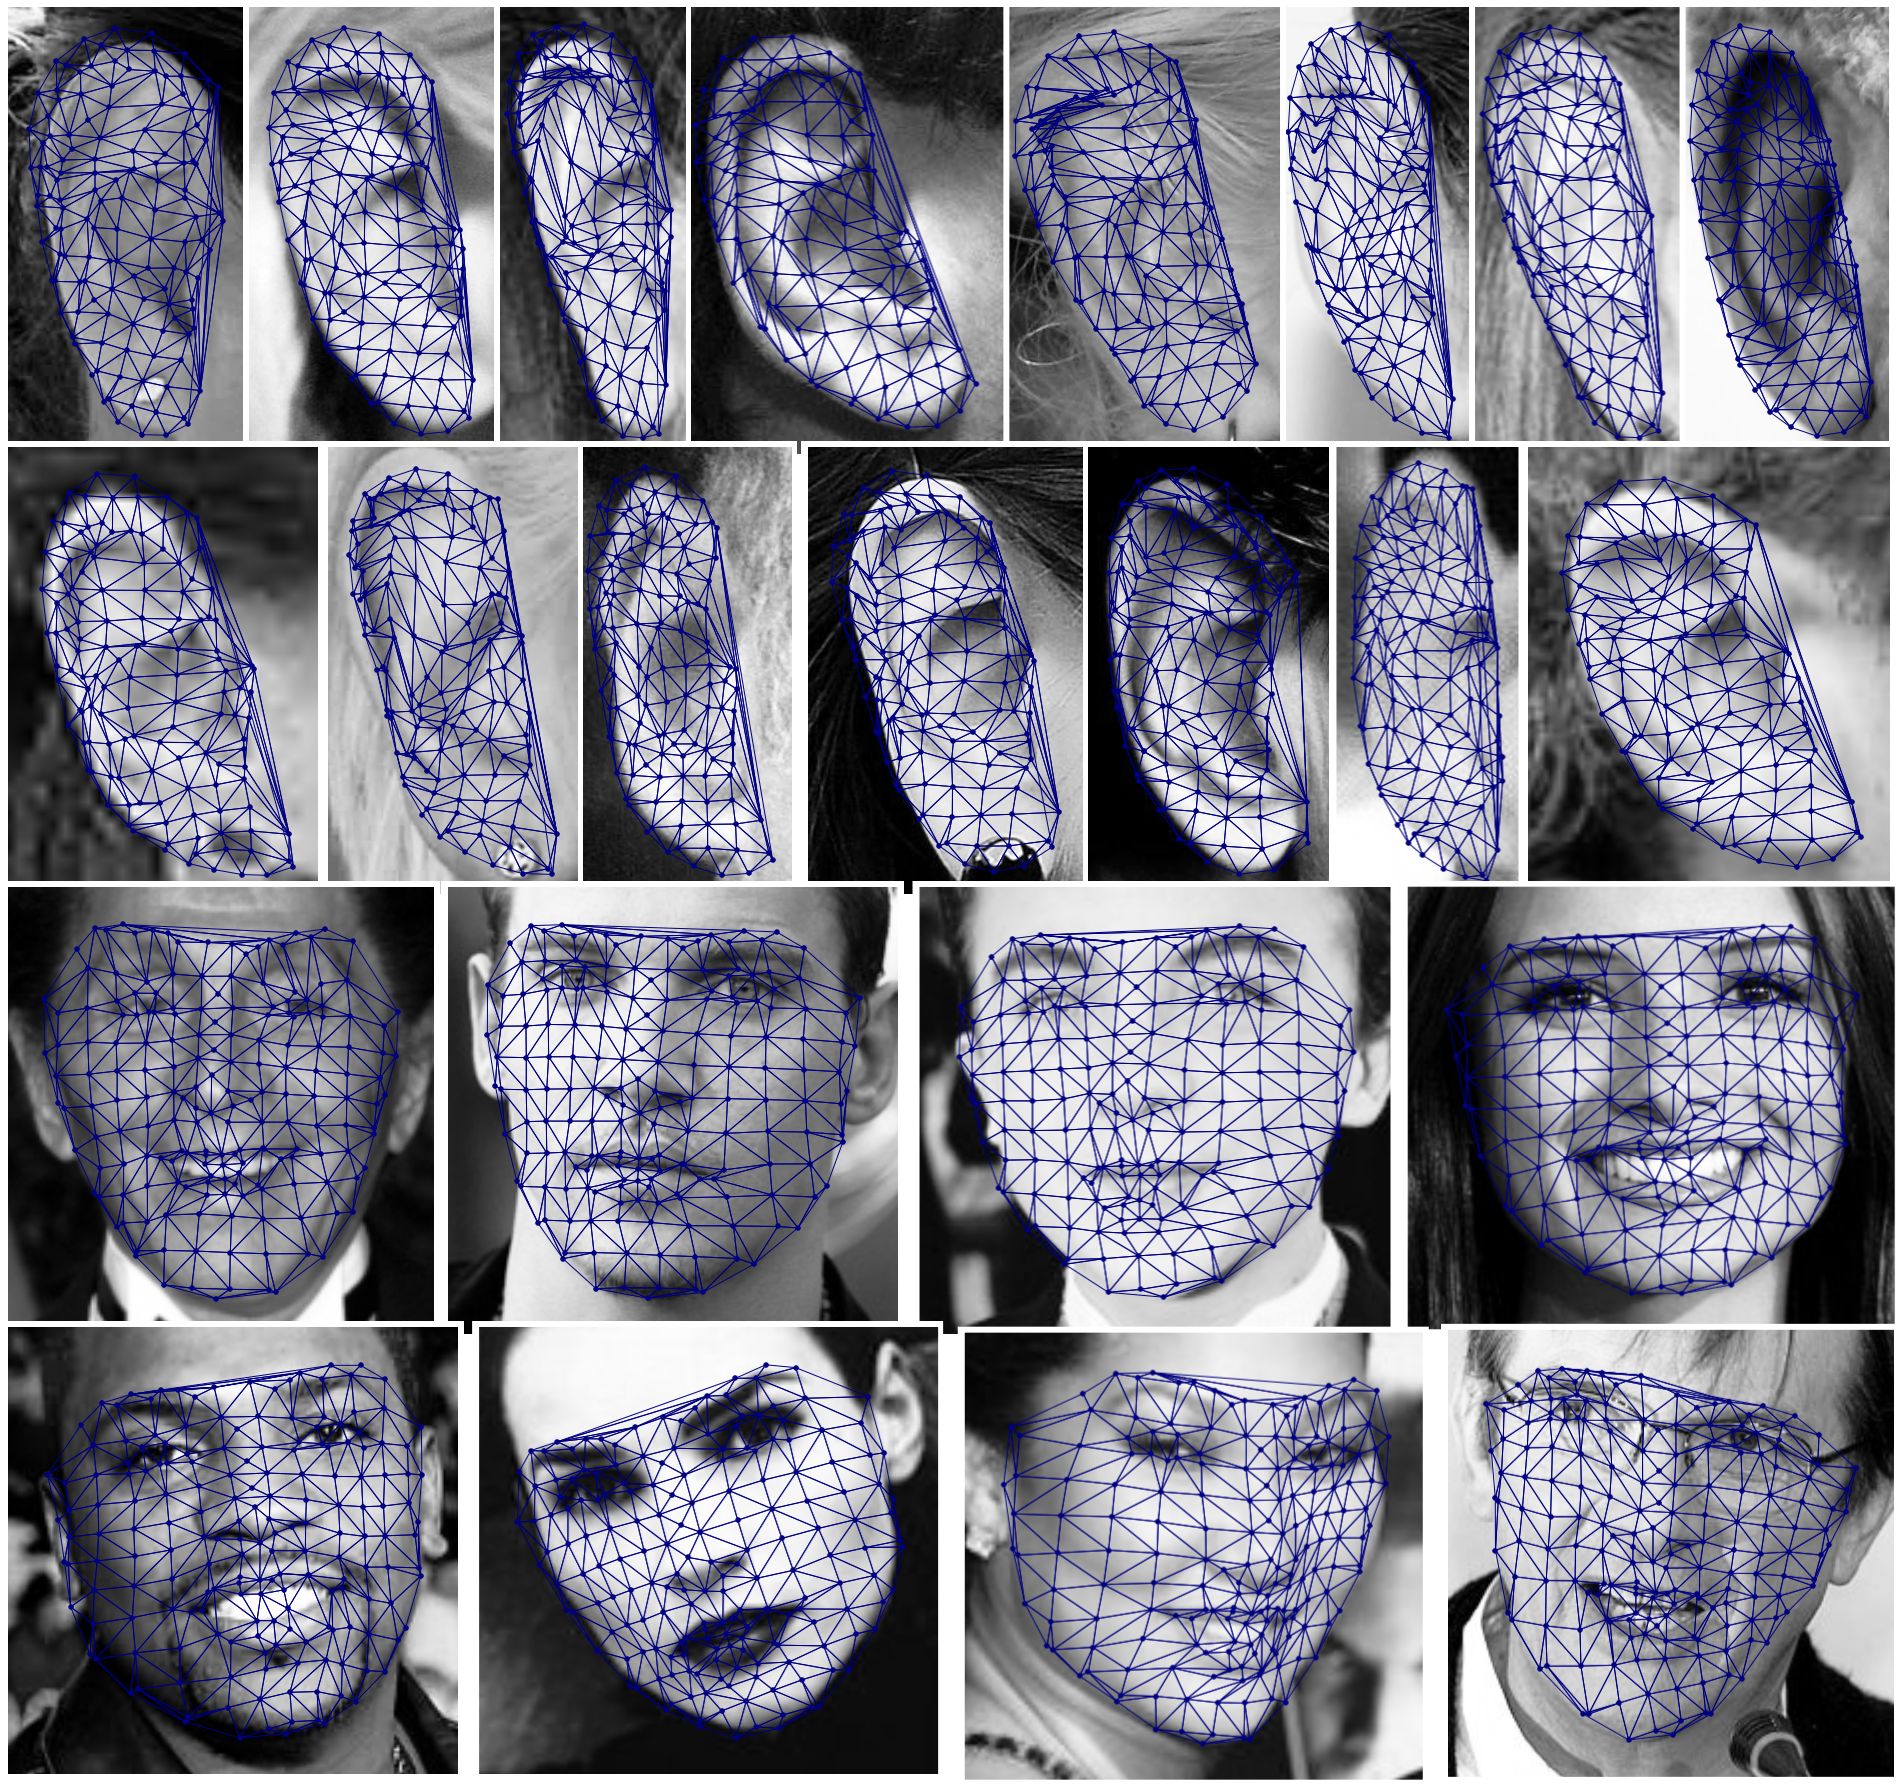
\includegraphics[width=0.5\textwidth]{supports/Fittings/fittings}
\caption{Result of fitting dAAMs on ears (first two rows) and faces (last two rows). A dense grid visualisation is used.}
\label{fig:fr}
\end{figure}



\section{Shape Model Analysis}
\label{sec:modelanalysis}


\begin{figure}[!b]
    \centering
    % \vspace*{-0.1in}
    \begin{subfigure}[b]{0.43\textwidth}
            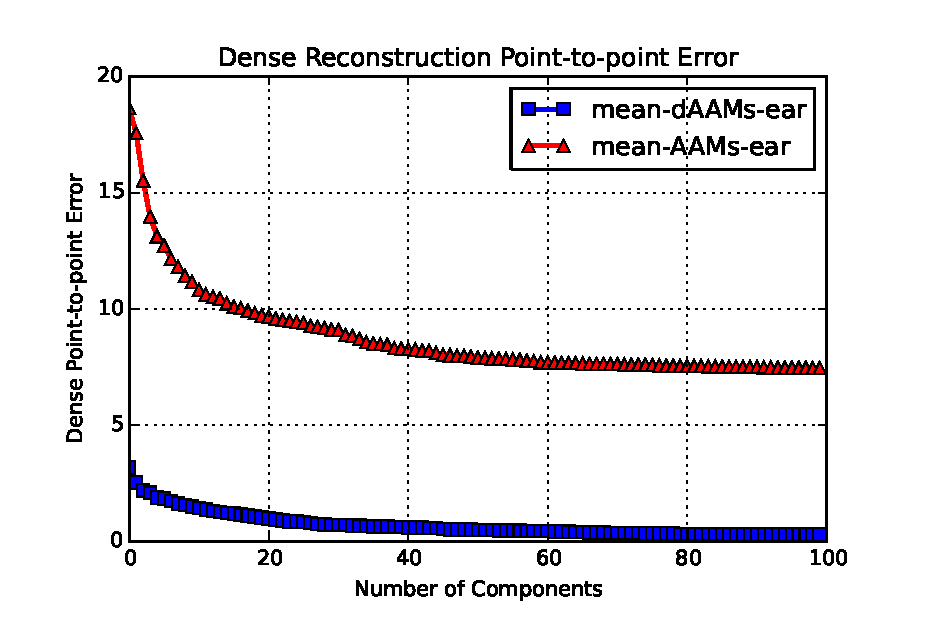
\includegraphics[width=\textwidth]{supports/Model_Analysis/sr_ear}
        %\caption{dAAMs dense shape reconstruction}
    \end{subfigure}
    \\
    \begin{subfigure}[b]{0.43\textwidth}
            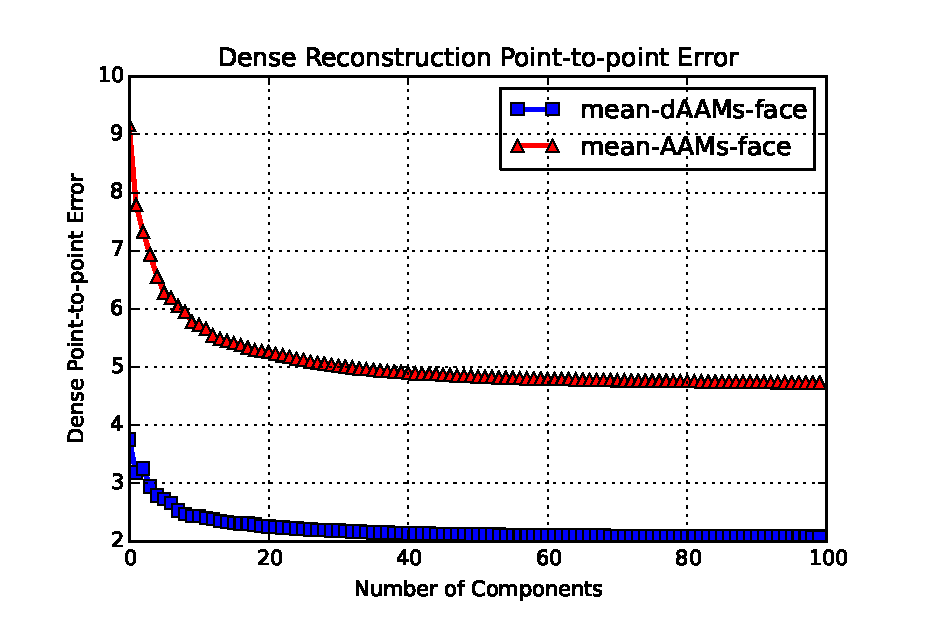
\includegraphics[width=\textwidth]{supports/Model_Analysis/sr_face}
        %\caption{AAMs dense shape reconstruction}
    \end{subfigure}
    \caption{Dense shape reconstruction errors for ears and faces. Top: results of reconstruction on ears, bottom: results of reconstruction on faces. The normalised point-to-point error is used an evaluation measure.}
    \label{fig:rc_face}
\end{figure}


We first investigate the reconstruction accuracy of AAMs and dAAMs in the shape space. In particular, given a ground-truth shape, we use the shape models from both AAMs and dAAMs to reconstruct the given shape densely. Since AAMs contain a sparse shape model, we densify it using a piecewise affine transformation, which is typically used in warping textures on to shape model too. Figure \ref{fig:rc_face} shows plots of dense shape reconstruction errors for ears and faces, for varying number of principal components kept. We observe that dAAMs significantly outperform classic AAMs on shape reconstruction. 


Furthermore, we explore the compactness of the built AAMs and dAAMs models. 
Figure \ref{fig:compact} demonstrates the variance explained as a function of the number of principal components. One can infer that dAAMs have a more compact shape model than AAMs, which leads to better reconstruction especially with few shape components.

\begin{figure}[!t]
    \centering
    \begin{subfigure}[b]{0.43\textwidth}
            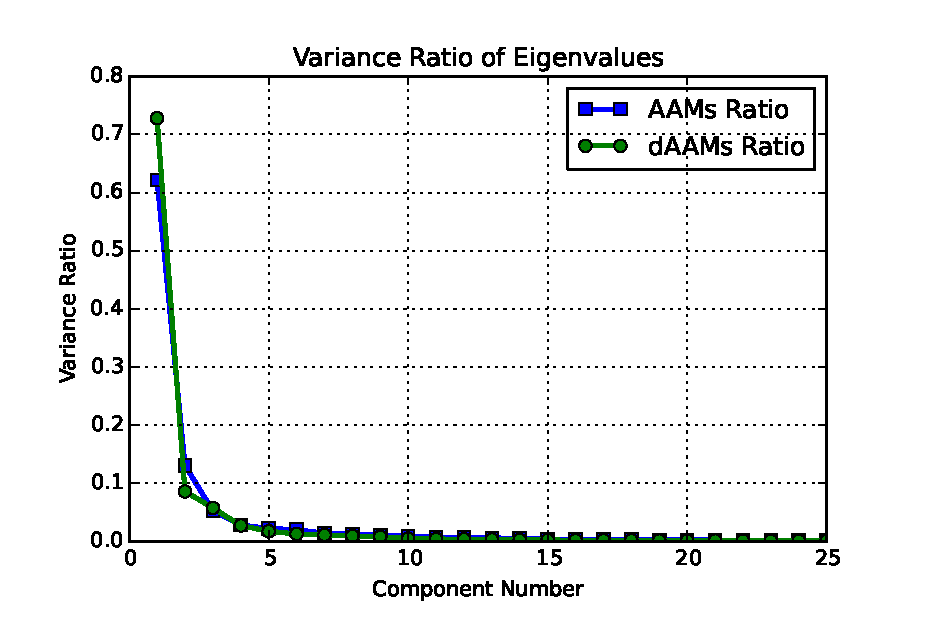
\includegraphics[width=\textwidth]{supports/Model_Analysis/var_ratio}
        %\caption{dAAMs vs AAMs Variance Ratio}
    \end{subfigure}
    \begin{subfigure}[b]{0.43\textwidth}
            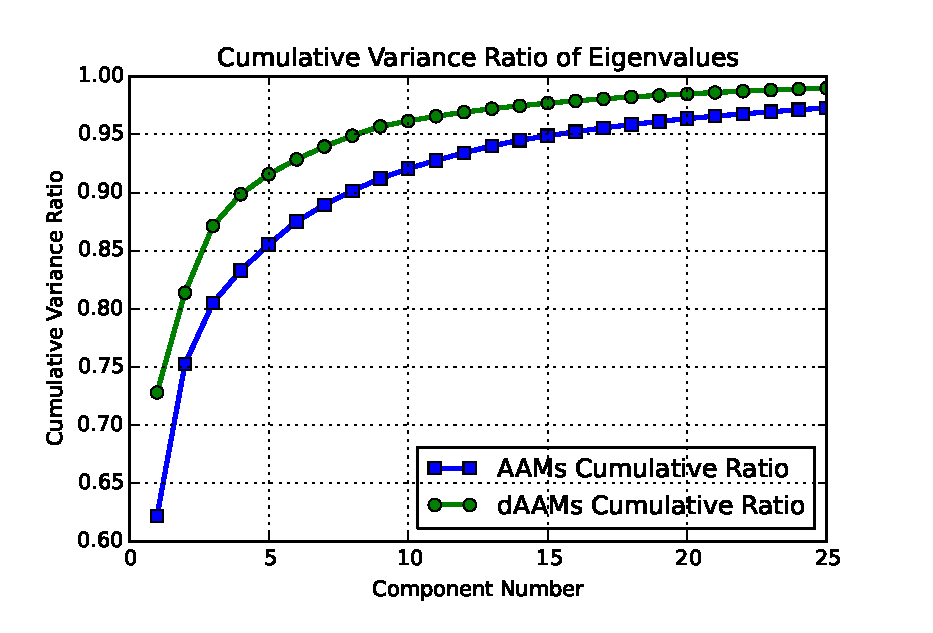
\includegraphics[width=\textwidth]{supports/Model_Analysis/cumu_var_ratio}
        %\caption{dAAMs vs AAMs Cumulative Variance Ratio}
    \end{subfigure}
    \caption{Variance explained by each principal component, for both dAAM and AAM models. Top: variance explained by each principal component. Bottom: cumulative plot of the variance explained as a function of the principal components.}
    \label{fig:compact}
\end{figure}

Finally, Figure \ref{fig:pcamodel} visualises the principal components of dAAMs for ears and faces. We observe that the variation of both shape and appearance captured by the model seem plausible.

\begin{figure*}[!t]
\centering
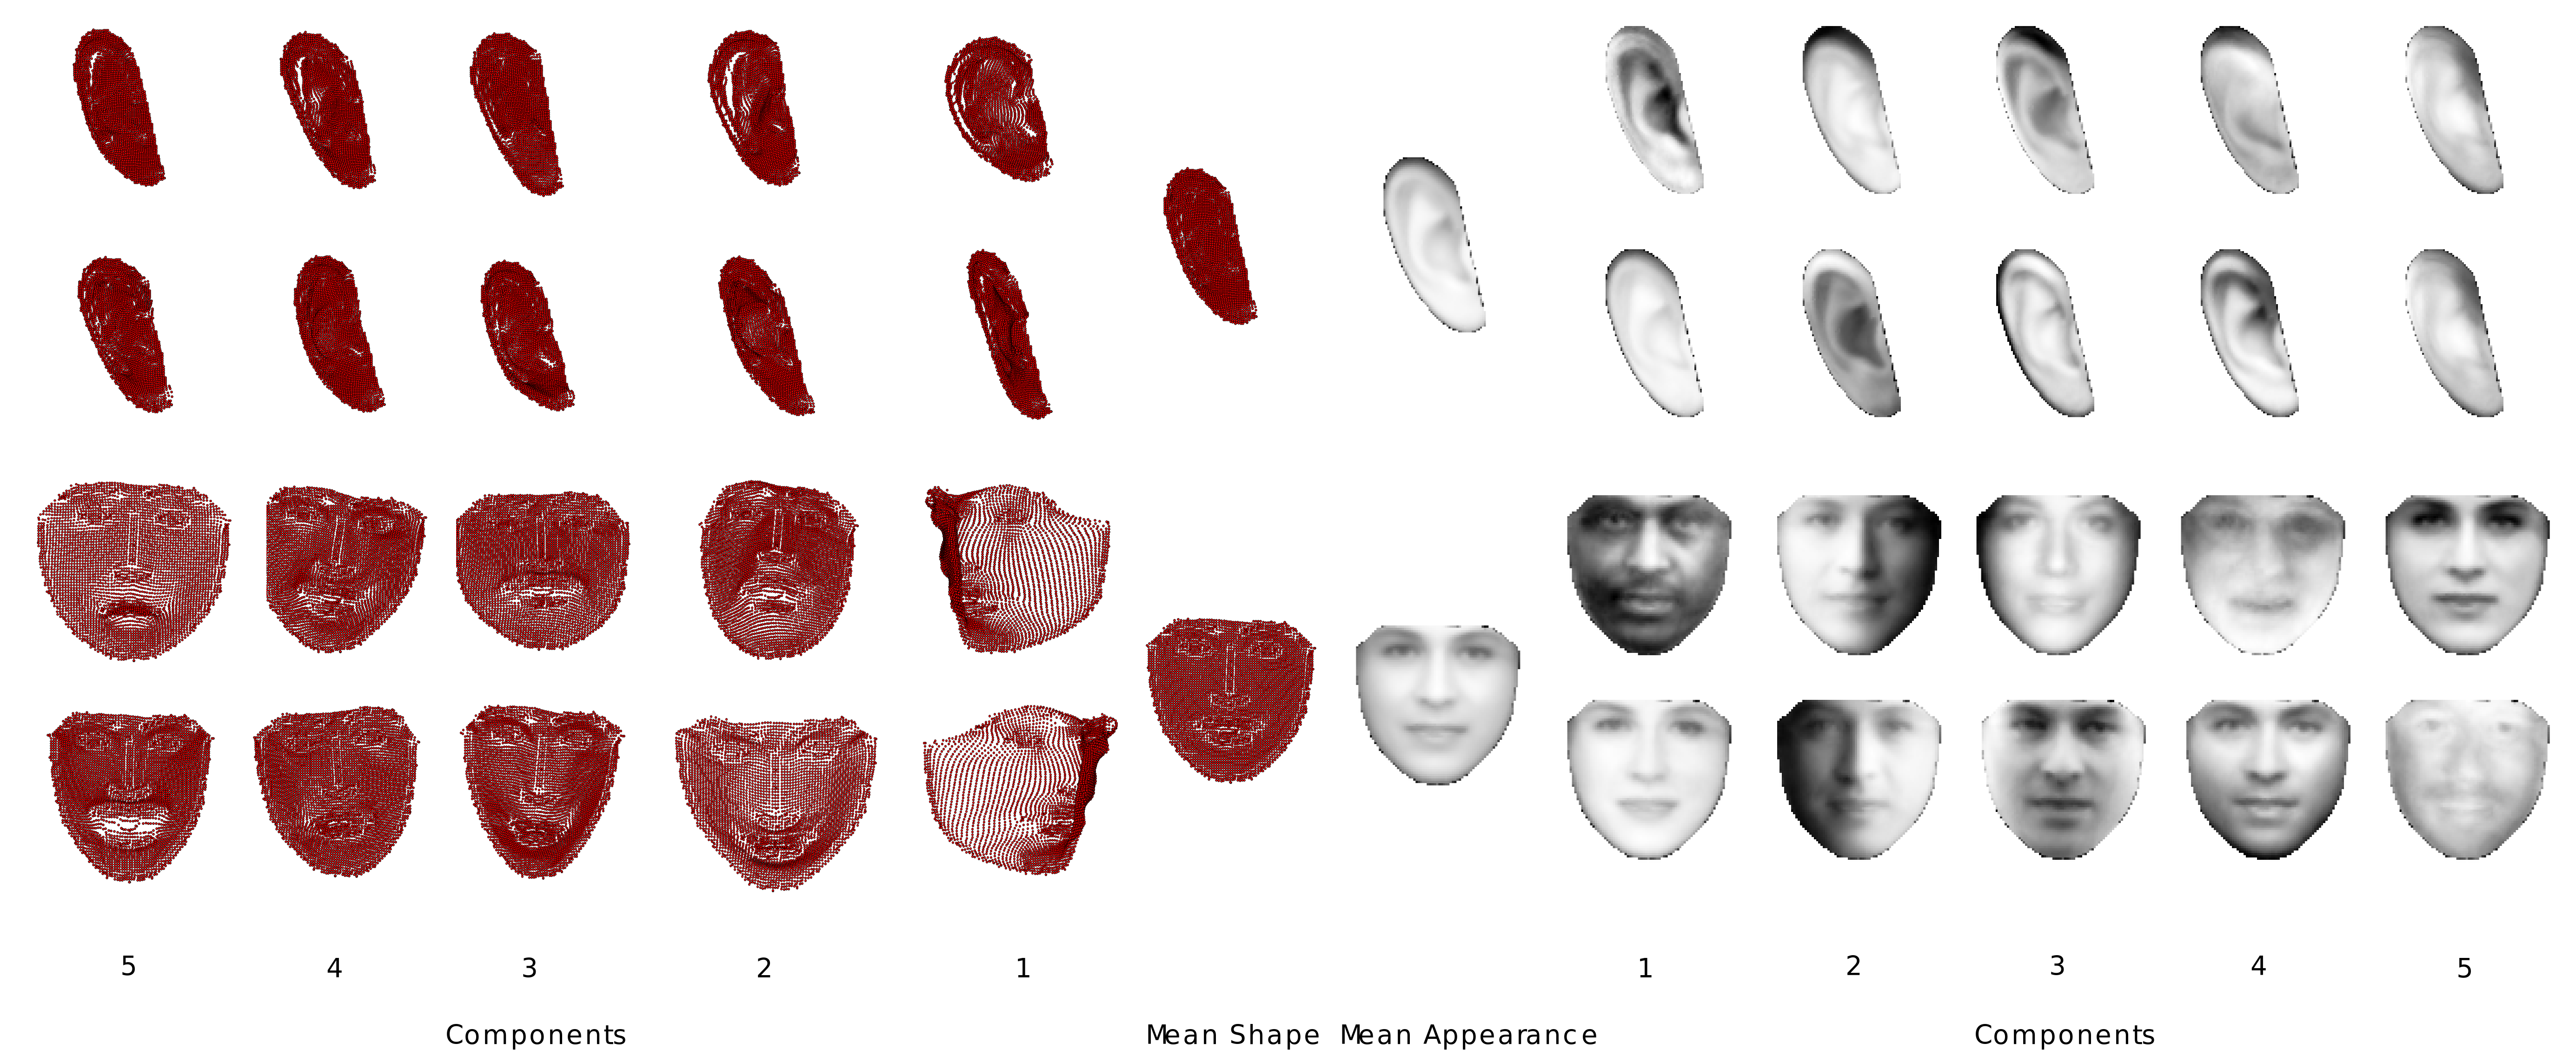
\includegraphics[width=\textwidth]{supports/Models/models}
\caption{Principal components of dAAMs built on ears (top) and faces (bottom). The mean (middle columns) as well as the first five principal components are visualised for both shape (left) and appearance (right). $\pm 3$ times the variance of the corresponding component is used in each case.}
\label{fig:pcamodel}
\end{figure*}




\section{Appearance Reconstruction}
\label{sec:reconstruct}

\begin{figure}[!b]
    \centering
    %\vspace*{-0.2in}
    \includegraphics[width=0.5\textwidth]{resources/Fig_Draw/draw}
    \caption{Synthesizing face images from caricature sketches. First column: caricature sketches. Second column: arbitrary chosen face images. Third and last column: sketch-based warping of images based on AAMs (third column) and dAAMs (last column).}
    \label{fig:draw}
\end{figure}

In this qualitative experiment, we show how the proposed pipeline can be used to generate novel modified instances of an object, e.g. caricatures. To be specific, firstly we manually craft a set of hand-drawn cartoon-like shape sketches. We then apply shape flow to align them with the reference frame. In this way, we establish dense correspondences of landmarks. Afterwards, we perform shape reconstruction using both AAMs and dAAMs. Finally, we warp the appearance from arbitrarily chosen faces on the reconstructed shape using either piecewise affine warp (in the case of AAMs) or shape flow (in the case of dAAMs). The corresponding results are shown in figure \ref{fig:draw}. We see that AAMs introduce more severe artifacts, especially on the areas of mouth and eyes, where nuanced information is missing or models are overly deformed. In contrast, dAAMs yield a significantly more plausible result.



\section{Segmentation using Dense AAM}
\label{sec:segmentation}

In this section, we present experiments of utilising our dense AAM for object segmentation. Two object classes, bottles and human bodies, are considered. For human bodies, we use images along with ground truth segmentation from Space-Time Actions dataset \footnote{\label{sta} \url{http://www.wisdom.weizmann.ac.il/~vision/SpaceTimeActions.html}}, which includes sequences with several human actions. We use ``jumping'' and ``sliding'' actions. As far as bottles are concerned, we use 500 high-resolution images that we collected and annotated using a newly-defined 50 point annotation scheme, as well as the curve annotations proposed in this paper. We randomly split these images into two disjoint sets of training (400) and testing (100) images. Bottle models were built using 400 training images while body models are built in terms of human actions (e.g. jumping), each having approximately 200 training images and 50 test images. 

\begin{figure}[!t]
    \centering
    \begin{subfigure}[b]{0.15\textwidth}
            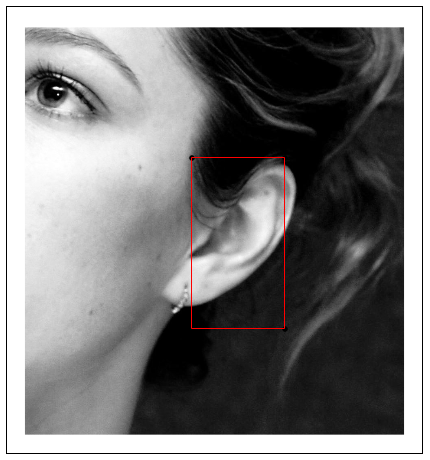
\includegraphics[height=\textwidth]{supports/Segmentation_Measure/ear}
        %\caption{Ear Initial Bounding Box}
    \end{subfigure}
    \begin{subfigure}[b]{0.15\textwidth}
            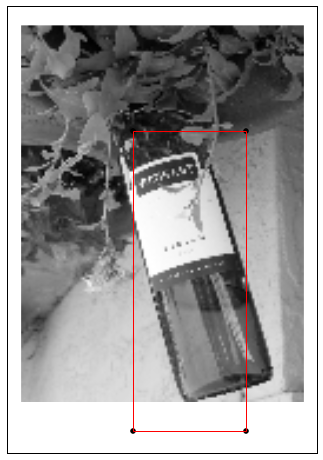
\includegraphics[height=\textwidth]{supports/Segmentation_Measure/bottle}
        %\caption{Bottle Initial Bounding Box}
    \end{subfigure}
    \begin{subfigure}[b]{0.15\textwidth}
            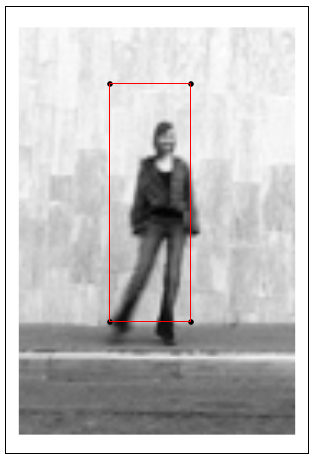
\includegraphics[height=\textwidth]{supports/Segmentation_Measure/body}
        %\caption{Body Initial Bounding Box}
    \end{subfigure}
    \caption{Examples of fitting initialisations used for the segmentation experiment. These are created by random perturbation of the ground-truth bounding box.}
    \label{fig:seg_init}
\end{figure}

Fitting dAAMs on test images yields dense landmarks that can be used to perform segmentation. In a real-world scenario, a simple object detector would be required to be applied prior to our pipeline to initialise the fitting. However, as a simple evaluation, we initialise the fitting by randomly perturbing the ground-truth bounding box with certain variance to simulate an object detector with implicit detection, see e.g.~Figure \ref{fig:seg_init}. Table  \ref{tab:seg_result} reports the segmentation precision, in case of fitting bottles and human bodies by adopting the proposed dAAMs pipeline.

\begin{table}[!h]
\small
\centering
\begin{tabular}{|l|c|c|c|}
\hline
\emph{Object}   & \emph{mean} & \emph{std} & \emph{median}\\
\hline\hline
Bottles         & 0.8125      & 0.1460     & 0.8414\\
Action - Jump   & 0.6102      & 0.0198     & 0.6099\\
Action - Slide  & 0.6444      & 0.0500     & 0.6501\\
\hline
\end{tabular}
\caption{Segmentation precision, in case of fitting bottles and human bodies by adopting the proposed dAAMs pipeline. The mean, standard deviation and median of the precision error are provided.}
\label{tab:seg_result}
\end{table}

% {\small
% \bibliographystyle{ieee}
% \bibliography{bib}
% }

\end{document}